% vim: set tw=78 sts=2 sw=2 ts=8 aw et ai:
\documentclass[12pt]{article}

\usepackage[paper=a4paper, top=2cm, bottom=3cm, left=2.5cm, right=2.5cm]{geometry}

\usepackage{ucs}
\usepackage{url}
\usepackage[utf8x]{inputenc}
\usepackage[english]{babel}
%\usepackage{hyperref}	  % use \url{http://$URL} or \href{http://$URL}{Name}
\usepackage{underscore}	  % underscores need not be escaped
\usepackage{subfigure}
\usepackage{verbatim}
\usepackage{float}
\usepackage{listings}
\usepackage{footnote}
\usepackage{perpage}
\MakePerPage{footnote}

% Support for including graphics
\usepackage{graphicx}
\DeclareGraphicsExtensions{.pdf,.png,.jpg}

\newcommand{\codename}{WSNsim }

\title{Implementing a new wireless sensor network simulator}

\author{Catalina Macalet, Sorin Dumitru\\
Automatic Control and Computers Faculty\\
University Politehnica of Bucharest\\
Splaiul Independenței nr. 313, Bucharest, Romania \\
\emph{\{catalina.macalet,sorin.dumitru\}@cti.pub.ro}}

\date{\today}

\begin{document}

\maketitle

\begin{abstract}
% vim: set tw=78 sts=2 sw=2 ts=8 aw et ai:
In this paper we report our research on some existing wireless network
simulators, namely NS-2, J-sim and TOSSIM and introduce \codename the 
wireless network simulator which we will develop hereafter, presenting its 
features and going into details regarding the architectural design and implementation.

All the surveyed simulators were not intended from the beginning to be
used for WSN simulations but rather modified later in order to simulate WNSs, 
\codename is to be used only 
for WSNs simulations, its design and
implementation being focused on taking the best decision for an accurate WSN
simulation. It will benefit from the experience of the already implemented
simulators using some of their key features and improving some others, but
it will also bring new features.


\end{abstract}

Keywords:
\begin{itemize}
  \item WSN
  \item Routing protocols
  \item NS-2/J-Sim/TOSSIM
  \item \codename
\end{itemize}

\section{Introduction}
\label{sec:introduction}
% vim: set tw=78 sts=2 sw=2 ts=8 aw et ai:

Wireless sensor networks consist of numerous autonomous sensors that are
capable of monitoring the environment in which they are placed with various
sensors. Such a network would be usefull for monitoring different things such
asas polution levels
in a city or poisonous gases or might be able to sense vibrations in order 
to predict an earthquake. 

A wireless sensor network will contain many nodes, anywhere from a couple of
hundred sensors to several thounds of nodes. Each of these nodes has one or
more sensors incorporated for getting data from the environment, the number of
sensors is limited
by the size and power consumption. Sensors also have a microcontroller 
to process the data from the sensor and a transceiver to be able send to some 
sink-node the data it collected. They are usually powered by some sort of battery 
although solar cells and capacitors have also been used.

Each sensor collects data from its location and sends it to the base station,
from where data from the whole network can be collected. A usual WSN is
presented in \figref{img:wsn}. It is very power
consuming to send data over long distances as the transceiver will need to
amplify the power more so this should be avoided if possible by sending data to
closer nodes. From this need of preserving the power 
arised a need of routing protocols for these
networks: instead of sending data directly to the base station, the nodes
group in an hierarchical way so that each node will send data to a cluster
head that is very close which then sends it to the base station or to a higher
order cluster head.

\fig{img/WSN.pdf}{img:wsn}{WSN}
%\includegraphics{img/WSN.pdf}

In this paper we will present some of the existing wireless network
simulators emphasizing what we believe to be their strenghts and weaknesses. 
In section NS-2 we discuss about NS-2 simulator, in section J-sim we present
J-sim and then we take a look at TOSSIM simulator. Based on these observations
we introduce in section \codename  the WSN simulator we will implement which
encompasses most of these simulators' strenghts and adds some new features
for wireless network simulators.


\section{Related Work}
\label{sec:relatedwork}
A large number of simulators exist to help research evaluate the behaviour of
wireless sensor networks. Some of this are general network simulators, like NS-2,
which has been adapted using modules to the area of wireless network simulators, others
where built especially for this use. There are also emulator of sensor nodes which can be
used to simulate network of small to medium size. Of these, we will take a look at NS-2, J-Sim
and TOSSIM.

\subsection{NS-2}
\label{subsec:ns2}

NS-2 was started as a version of the REAL network simulator. It is currently at its 
second iteration while its third(NS-3) is in active development and in a usable state.
Work on it started working in 1989 and it was quicly adopted by the research community.
Among the contributors to NS-2 have been Sun Microsystems, Xerox and Carnegie Mellon 
university. 

NS-2 simulations are written in a combination in of C/C++ and OTCL. C and C++ is 
used for definig protocols and libraries while OTCL is used to define and control
the simulation.

Basic support for mobile nodes in NS-2 is added through the MobileNode class. This extends
the generic Node class and adds support for mobilty of the node and the capability to
send and receive messages on a wireless medium. 
Example commands to set the position and the movement of a node:
\lstset{numbers=none,language=C,caption=Commands to set the position and movement of a node,label=lst:saddrule}
\begin{lstlisting}
	$node set X_ <x>
	$node set Y_ <y>
	$node set Z_ <z>
	$ns at $time $node setdest <x> <y> <speed>
\end{lstlisting}
As it can be seen, although we can specify the position of the node in three dimensions,
only two are used for the mobilty of nodes.

Support for simulating wireless sensor networks in NS-2 has been added by the 
MANNASIM project\footnote{\url{http://www.mannasim.dcc.ufmg.br/}}. It comes as
a patch for NS-2 which add support for wireless sensors. It includes a number of
new classes:
\begin{itemize}
	\item SensorNode class which is built on top of NS-2's MobileNode 
to include characteristics specific to wireless sensors such as power 
consumption, memory and cpu.
	\item BatteryClass, extenden from EnergyModel, which is used to simulate
the battery of a node
	\item DataGenerator, used for simulating the data with which the sensor is
working. Can be used to simulate programmed, continuous, on demant and event driven
data sources.
\end{itemize}

An important part of wireless sensor simulators is the environment in which the sensors
are placed. It can affect the power needed to transmit a packet, the placement of nodes
and the accurate determination of the position of neighbouring nodes. It is possible to
simulate some of these in NS-2 but not in a detailed way.

\subsection{J-Sim}
\label{subsec:jsim}
J-sim\footnote {original web site \url{http://j-sim.cs.uiuc.edu/}, moving to 
\url{http://sites.google.com/site/jsimofficial/}} is a component based development
environment

\subsection{TOSSIM}
\label{subsec:tossim}
TOSSIM\cite{tossim} is a simulator for TinyOS sensor networks.
All the protocol and systems simulated using TOSSIM are written in nesC \cite{nesC},
an extension to C programming language designed to meet the specification and 
restrictions of TinyOS. At a first glance this might seem a disadvantage, but 
the code can then be reused on real-world motes running TinyOS
without further changes.
\\
TOSSIM provides debugging facilities having several debugging modes 
(such as boot, clock,task,led,...) some of which are being used in TinyOS code
and others are reserved for applications components. Compiling TinyOS for mote
hardware removes the debug statements.
It also provides support for network monitoring and packet injection
through SerialForwarder\footnote{\url{http://docs.tinyos.net/index.php/Mote-PC_
serial_communication_and_SerialForwarder}}, the TinyOS interface tool.
\\
For radio communication, TOSSIM provides two modes: the simple mode when bits
are transmitted without errors regardless of the distance between of the transmitting
motes, and the lossy mode, when for every pair of motes a number between 0 and 1 
denotes the probability with which every received bit will be corrupted. These 
mapping are defined in a configuration file which is given as an argument at boot
time. The values specified in this configuration file can be changed at runtime
by sending control messages through a TCP socket to TOSSIM.
 Except for this lossy mode, the degradation of signal can be modeled using
LossyBuilder which limits the transmitting area of every mote to a radius of 50
 feet and, at the same time, takes into consideration the rates defined as 
described above.
The values read from ADC are 10 bit values generated either random or generic, set
by default to random as well but which can be controlled through control messages.
\\
TOSSIM models the EEPROM memory with a memory-mapped file which, by default, is
unmapped at the end of simulation but it can be configured to be persisten if a
named file is specified at run-time.
\\
TinyViz is an extensible GUI which, besides offering a visual layout of the 
WSN, offers support for debugging and interaction with TOSSIM. Also, traffic can
be seen using TinyViz and extra functionality added through plugins
\footnote{\url{http://www.tinyos.net/tinyos-1.x/doc/tutorial/lesson5.html}}.
A model of a TOSSIM network is defined by the following structure:
\begin{lstlisting}
typedef struct {
    void(*init)();
    void(*transmit)(int, char); //int moteID, char bit
    void(*stop_transmit)(int);  //int moteID
    char(*hears)(int);          //char bit, int moteID
    bool(*connected)(int,int);  //int moteID1, int moteID2
    link_t*(*neighbors)(int);   //int moteID
} rfm_model;
\end{lstlisting}




\section{\codename}
\label{sec:simulator}
\subsection{Architecture}
\begin{center}
	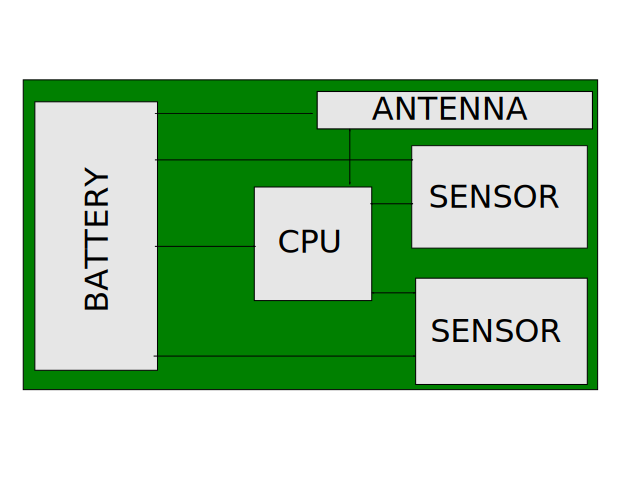
\includegraphics[scale=0.6]{img/board.pdf}
\end{center}
\subsection{Components}
\subsection{Environment}


\section{Conclusion and Further Work}
\label{sec:conclusion}
% vim: set tw=78 sts=2 sw=2 ts=8 aw et ai:

While the simulators investigated in this paper are very useful, we believe
that there is room for improvement. Most of them are generic simulators
adapted for simulating wireless sensor networks. 
We believe that a simulator built from the beginning, having in mind that it
will be used for wireless sensors, will increase its usability and make it
possible for it to be useful in more circumstances.
We propose the following plan to build the simulator described above in a couple
of phases.
We will begin by fully designing the component architecture and basic node
structure. We will build template components and create the necessary framework to integrate them 
into a sensor node. Next we will create the necessary framework for the nodes
to communicate. 
After being able to simulate a wireless sensor network, we will implement some
routing protocols, such as LEACH and TEEN, and based on the results of the
simulation of these protocols, we will determine \codename's performance.
The final step is integrating the environment simulation into the simulator.
We will augment the simulator with environment simulation as described in the paper.
%\begin{itemize}
%  \item Component architecture and basic node structure. We will build
%  template components and create the necessary framework to integrate them
%  into a sensor node.
%  \item Comunication between nodes. Create the neccessary framework to make
%  two nodes communicate.
%  \item Implement some routing procols. To evaluate our simulator we will
%  implement some routing procols(LEACH, TEEN) in it and see it's performance
%  \item Environment simulation. Will augment the simulator with environment
%  simulation as described in the paper.
%\end{itemize}


\section*{Acknowledgment}
\label{sec:acknowledgment}

The authors would like to thank XYZ for their support and dedication.

\bibliographystyle{abbrv}
\bibliography{report}

\end{document}
